\documentclass{beamer}
% \documentclass[notes]{beamer}

\usepackage{graphicx}       % Extended support for \includegraphics
\usepackage{tikz}           % Powerful drawing package, part of pgf
\usepackage{url}            % \url command for decent line breaks in urls
\usepackage{array}          % Improved array support
\usepackage{textcomp}       % Extra symbols

% Enable this for summary printout
% \usepackage{pgfpages}\pgfpagesuselayout{4 on 1}[
%     a4paper, landscape, border shrink=2mm]


\usetikzlibrary{matrix}             % Grid placement
\usetikzlibrary{positioning}        % Anchor placement support
\usetikzlibrary{calc}               % Coordinate calculations
\usetikzlibrary{shapes.geometric}   % cylinder
\usetikzlibrary{shapes.symbols}     % cloud
\usetikzlibrary{shapes.arrows}      % arrow shapes
\usetikzlibrary{shapes.multipart}
\usetikzlibrary{fit}                % Fitting outline to shape
\usetikzlibrary{shadows}
\usetikzlibrary{arrows}

% Common TikZ definitions
\tikzset{
    % This seems a reasonably comfortable arrow shape
    >=stealth,
%
    % Used for creating an exact fit to an existing list of objects
    tight fit/.style={fit=#1, inner sep=0, line width=0},
%
    % Draws a reasonably sensible looking disk icon
    disk icon/.style={
        draw, thick, cylinder, shape border rotate=90,
        minimum width=1cm, minimum height=.75cm},
%
    % A moderate highlighting fill
    background fill/.style={fill=black!15},
    % A gentle highlighing fill
    highlight fill/.style={fill=green!60!blue!20},
    % A rather darker fill for shadows
    shadow fill/.style={fill=gray}}

% It's handy to have a foreground and background layer available.
\pgfdeclarelayer{background}
\pgfdeclarelayer{foreground}
\pgfsetlayers{background,main,foreground}


%\usetheme{Singapore}
\usetheme{dlstalk}
\setbeamertemplate{navigation symbols}{}
\setbeamertemplate{items}[circle]


% \title{A new Fast Data Logger and Viewer at Diamond:\\the FA Archiver}
\title[The FA Archiver]{A Fast Acquisition Archiver}
\author{Michael Abbott}
\institute[Diamond]{Diamond Light Source \\ \url{michael.abbott@diamond.ac.uk}}
% \date{13th October 2011}
% \date{ICALEPCS 2011}
% \date{29th September 2011}
\date{ICALEPCS 2011}




\begin{document}

\begin{frame}
\titlepage
\end{frame}

% Place date discreetely on every slide.
\setbeamertemplate{footline}{\hspace*{\fill}\insertdate}


\begin{frame}\frametitle{The Fast Acquisition Archiver}

The FA archiver captures $X,Y$ position data from a network of electron beam
position monitors (EBPMs) and other sources at 10\,kHz, maintains a rolling
historical record and rebroadcasts the complete data stream to all interested
parties.

\begin{itemize}

\item 256 $X,Y$ position updates every 100\,\textmu s, sustained 20\,MB/s.

\item At Diamond we archive the last 4\textonehalf{} days of orbit position.

\item Any number of clients (limited by network connection to archive server)
can read the archive and subscribe to the rebroadcast live data stream.

\end{itemize}
\end{frame}



\begin{frame}\frametitle{The Fast Acquisition Archiver}
\begin{center}
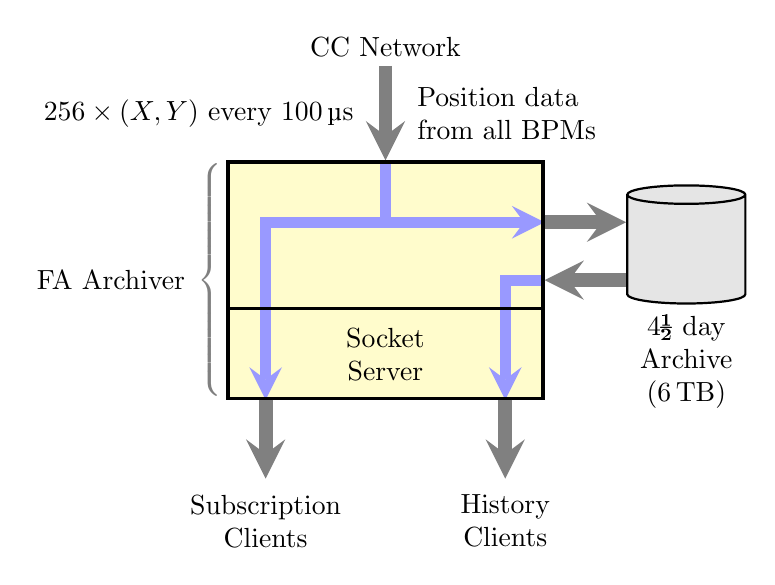
\begin{tikzpicture}

\tikzset{
    accent/.style={color=blue!40, line width=4pt},
    highlight/.style={fill=yellow!20}}

\path (0,0)
    node (cc) {CC Network}
    [draw, line width=5pt, gray, ->] (cc.south) -- ++(0,-12mm)
    coordinate (input)
    node [midway, left, black, xshift=-2mm]
        {$256\times(X,Y)$  every 100\,\textmu{}s}
    node [midway, right, black, align=left, xshift=2mm]
        {Position data\\from all BPMs};
\node (archiver) [
        draw, very thick, rectangle, anchor=north,
        label={[xshift=-4mm]left:FA Archiver},
        minimum width=40mm, minimum height=30mm] at (input) {};
\path [gray] node [fit=(archiver), inner sep=0pt, left delimiter=\{] {};

\draw[very thick] (archiver.-10) -- (archiver.-170);
\path (archiver.-10) -- (archiver.south west)
    node [midway, align=center] {Socket\\Server};

\draw [line width=5pt, gray, ->] (archiver.-135) -- +(0, -10mm)
    node [black, anchor=north, align=center] {Subscription\\Clients};
\draw [line width=5pt, gray, ->] (archiver.-45) -- +(0, -10mm)
    node [black, anchor=north, align=center] {History\\Clients};

\begin{pgfonlayer}{background}
\path[highlight] (archiver.north west) rectangle (archiver.south east);
\draw[accent, ->] (archiver.north) |- (archiver.20);
\draw[accent, ->] (archiver.0) -| (archiver.-45);
\draw[accent, ->] (archiver.north |- archiver.20) -| (archiver.-135);
\end{pgfonlayer}

\node (disk) [disk icon, fill=black!10,
    minimum height=15mm, minimum width=15mm, xshift=18mm,
    label={[align=center]below:4\textonehalf{} day\\Archive\\(6\,TB)}]
    at (archiver.10) {};
\draw [line width=5pt, color=gray, ->]
    (archiver.20) -- (archiver.20 -| disk.west);
\draw [line width=5pt, color=gray, <-]
    (archiver.0) -- (archiver.0 -| disk.west);

\end{tikzpicture}

\end{center}
\end{frame}



\begin{frame}\frametitle{Getting Fast BPM Data}

The archiver connects to the Diamond Communication Controller (CC) fast orbit
feedback network.

\begin{itemize}

\item All storage ring EBPMs are connected to CC network.

\item Network is based on synchronous broadcast via store and forward: every
100\,\textmu s, every node has complete position information.

\item Easy to add new nodes, both as listeners and contributors.

\item FA archiver ``piggy backs'' on existing feedback infrastructure.

\end{itemize}

\end{frame}



\begin{frame}
\frametitle{Communication Controller Network Topology}
\includegraphics[width=\linewidth]{fofb}
\end{frame}



\begin{frame}\frametitle{Hardware Requirements for FA Archiver}
\begin{itemize}

\item Need FPGA with Rocket I/O and Diamond Communication Controller FPGA image
to connect to CC network.

\vspace{2pt}
Diamond CC FPGA image is freely available from Diamond subject to a standard
``Memorandum of Understanding''.

\item FA Archiver uses Xilinx PCI express FPGA development board to connect to
CC network.

\vspace{2pt}
Unfortunately this board is large and abnormally tall, so won't fit in all PCs.

\item Archiver works on relatively low spec hardware; we use a dual core Dell
R200 1U server.


\end{itemize}

\end{frame}




\begin{frame}\frametitle{FA Archiver in Context}
\begin{center}
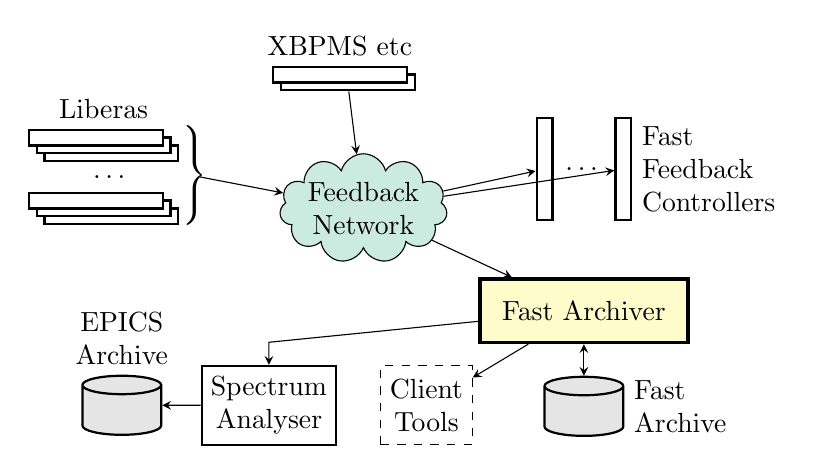
\begin{tikzpicture}

% Nice puffy cloud representing the FA network
\path[xshift=27mm, yshift=5mm, thin]
    node[draw, cloud, aspect=2, cloud puffs=11, inner sep=0pt, highlight fill,
        align=center]
        (fa network) {Feedback\\Network};

% Draw a stack of rectangles representing the liberas
\path[xshift=-5mm, yshift=12mm,
    libera/.style={
        draw, rectangle, thick, fill=white, inner sep=0,
        minimum width=1.7cm, minimum height=2mm}]

    { [current point is local=true]
    node[libera] {}
    ++(-1mm,1mm) node[libera] {}
    ++(-1mm,1mm) node[libera] (top libera) {}
    }

    +(0mm,-3mm) node {\dots}
    ++(0mm,-8mm)
    { [current point is local=true]
    node[libera] (bottom libera) {}
    ++(-1mm,1mm) node[libera] {}
    ++(-1mm,1mm) node[libera] {}
    }
    node[tight fit=(top libera) (bottom libera),
        right delimiter=\}, label=north:Liberas] (liberas) {};

\draw[->] ($(liberas.east)+(2.6mm,0)$) -- (fa network);

\path[xshift=25mm, yshift=21mm,
    libera/.style={
        draw, rectangle, thick, fill=white, inner sep=0,
        minimum width=1.7cm, minimum height=2mm}]

    node[libera] (xbpms) {}
    ++(-1mm,1mm) node[libera, label=north:XBPMS etc] {};

\draw[->] (xbpms) -- (fa network);


% Fast feedback controllers
\path[xshift=50mm, yshift=10mm,
    controller/.style={
        draw, rectangle, thick, inner sep=0,
        minimum width=2mm, minimum height=13mm}]

    node[controller] (left controller) {}
    ++(5mm,0mm) node {\dots}
    ++(5mm,0mm) node[controller,
        label={[align=left]right:Fast\\Feedback\\Controllers}]
    (right controller) {};

\draw[->] (fa network) -- (left controller);
\draw[->] (fa network) -- (right controller);

% The archiver saving into the archive store
\path[xshift=5.5cm, yshift=-8mm]
    node[draw, very thick, rectangle, inner sep=8pt, fill=yellow!20]
        (archiver) {Fast Archiver}

    node[disk icon, below=4mm of archiver, fill=black!10] (fa archive) {}
    node[tight fit=(fa archive),
        label={[align=left]right:Fast\\Archive}] {}
    [draw,<->] (archiver) -- (fa archive);

\draw[->] (fa network) -- (archiver);

% Spectrum analyser saving into EPICS archive
\path[xshift=15mm, yshift=-20mm]
    node[draw, thick, rectangle, align=center, minimum height=10mm]
        (spectrum) {Spectrum\\Analyser}

    node[disk icon, anchor=shape center, fill=black!10,
        label={[align=center]above:EPICS\\Archive}]
        (epics archive) at ($(spectrum.west)-(10mm,0)$) {}
    node[tight fit=(epics archive)] (epics archive fit) {}

    [draw,->] (spectrum) -- (epics archive fit);

\draw[->] (archiver) -- ($(spectrum)+(0,8mm)$) -- (spectrum);

% Client tools
\path[xshift=35mm, yshift=-20mm]
    node[draw, rectangle, align=center, minimum height=10mm, dashed]
        (client tools) {Client\\Tools};

\draw[->] (archiver) -- (client tools);

\end{tikzpicture}

% vim: set filetype=tex:

\end{center}
\end{frame}



\begin{frame}\frametitle{FA Archiver Architecture}

\begin{itemize}

\item Very regular data feed: fixed size updates at fixed intervals.
Makes archiver design much simpler than an EPICS archiver.

\item The historical archive is fixed length, determined by disk size.  Old data
is discarded as new data arrives.

\item Data is reordered for fast read access before storage to disk.

\item Overview data (decimated by binning) also stored.

\item Archive indexed by timestamp of arrival of CC data.

\end{itemize}
\end{frame}



\begin{frame}
\frametitle{FA Archiver Architecture}
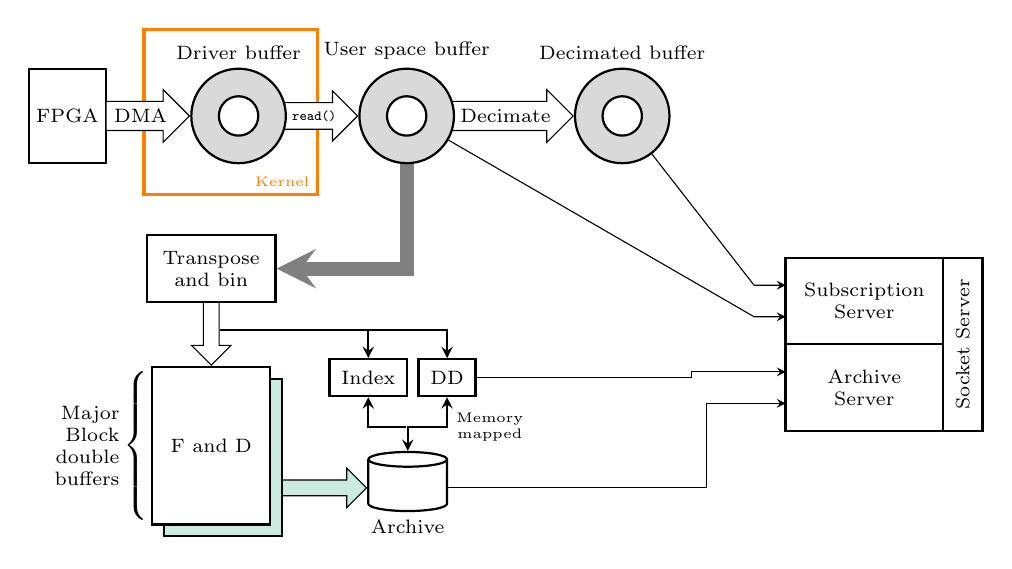
\begin{tikzpicture}[
    single arrow head extend=1.5mm]
\scriptsize

% Draws a circular buffer with name #1 east of #2 with top label #3 and centre
% label #4
\newcommand{\buffer}[3]{
\begin{pgfonlayer}{foreground}
\path
    node [draw, thick, circle, background fill,
        minimum width=12mm, anchor=west,
        label={above:#3}] (#1) at (#2.east) {}
    node [draw, thick, fill=white, circle, minimum width=5mm] at (#1) {};
\end{pgfonlayer}
}

% Sniffer device and its connections
\node [draw, thick, anchor=west, minimum height=12mm] (fpga) {FPGA};
\node [draw, single arrow, anchor=west, fill=white]
    (dma) at ($(fpga.east)-(0.2mm,0)$) {DMA};

% Device driver
\buffer{device buffer}{dma}{Driver buffer}
\node [draw, single arrow, anchor=west, fill=white]
    at ($(device buffer.east)-(0.4mm,0)$)
    (device) {\tiny\texttt{read()}};

\begin{pgfonlayer}{background}
\draw [orange, very thick] ($(device buffer)+(-12mm,11mm)$)
    rectangle ($(device buffer)+(10mm,-10mm)$);
\node [orange, anchor=south east, font=\tiny]
    at ($(device buffer)+(10mm,-10mm)$) {Kernel};
\end{pgfonlayer}


% Central raw circular buffer and decimated buffer
\buffer{raw buffer}{device}{User space buffer}
\node [draw, single arrow, anchor=west] at ($(raw buffer.east)-(0.4mm,0)$)
    (decimate) {Decimate};
\buffer{decimated buffer}{decimate}{Decimated buffer}


% Transposing to in-memory disk buffer
\node [draw, thick, anchor=north west, inner sep=2mm, align=center]
    at (15mm, -15mm)
    (transpose) {Transpose\\and bin};
\path [draw, line width=5pt, color=gray, ->] (raw buffer) |- (transpose);
\node [draw, single arrow, rotate=-90, anchor=west, minimum height=8mm]
    (transpose arrow) at ($(transpose.south)+(0,0.2mm)$) {};
\begin{pgfonlayer}{foreground}
\node [draw, thick, fill=white,
    minimum height=20mm, minimum width=15mm, anchor=north, align=center,
    left delimiter=\{, copy shadow={
        shadow xshift=1.5mm, shadow yshift=-1.5mm, highlight fill},
    label={[align=right, xshift=-3mm]left:Major\\Block\\double\\buffers}]
    (major block) at (transpose arrow.east) {F and D};
\end{pgfonlayer}


% Archive on disk and in memory
\node [draw, single arrow, anchor=west, minimum width=1mm, minimum height=12mm,
    highlight fill]
    (archive arrow) at (major block.325) {};
\node [disk icon, anchor=west, label={below:Archive}]
    (archive) at (archive arrow.east) {};

\node [draw, thick, inner sep=1.5mm]
    (index) at ($(archive)+(-5mm,14mm)$) {Index};
\node [draw, thick, inner sep=1.5mm] (dd) at ($(archive)+(+5mm,14mm)$) {DD};

\draw [->, thick] (transpose arrow) -| (index);
\draw [->, thick] (transpose arrow) -| (dd);
\node [inner sep=0pt, line width=0] (via) at ($(archive.north)+(0,3mm)$) {};
\draw [<-, thick] (index) |- (via);
\draw [<->, thick] (dd) |- (via.center) -- (archive);

\node [right=5mm of via, align=center, font=\tiny] {Memory\\mapped};


% Socket Server
\path [draw, thick]
    (\linewidth, -40mm) rectangle ++(-5mm,22mm) coordinate (a)
    node [rotate=90, pos=0.5] {Socket Server}
    rectangle ++(-20mm,-11mm) coordinate (b)
    node [pos=0.5, align=center] {Subscription\\Server}
    rectangle ++(20mm,-11mm) coordinate (c)
    node [pos=0.5, align=center] {Archive\\Server}
    node [tight fit=(a) (b), align=center] (subscription server) {}
    node [tight fit=(b) (c), align=center] (archive server) {};

\draw [<-] ($(subscription server.west)+(0,-2mm)$)
    -- +(-4mm,0) -- (raw buffer);
\draw [<-] ($(subscription server.west)+(0,2mm)$)
    -- +(-4mm,0) -- (decimated buffer);
\draw [<-] ($(archive server.west)+(0,2mm)$) -- +(-12mm,0) |- (dd);
\draw [<-] ($(archive server.west)+(0,-2mm)$) -- +(-10mm,0) |- (archive);


\end{tikzpicture}

% vim: filetype=tex:

\end{frame}



\begin{frame}\frametitle{Archiver Services}

The FA archiver provides the following data over TCP/IP to any connecting
machine:

\begin{itemize}

\item Subscription to any subset of the complete CC data stream.
\note{If the client doesn't take data rapidly enough it will be disconnected by
the server.}

\item Subscription to any subset of the complete CC data stream decimated by a
factor of 10.
\note{

This data stream is spectrally flat and alias free up to around 400\,Hz.}

\item Access to any part of the historical archive, both full and decimated,
indexed by timestamp.

\end{itemize}
\end{frame}



\begin{frame}\frametitle{Decimated Archive Data}

To help with reviewing beam movement over hours or days, the archived data is
also stored in decimated format.

\begin{itemize}

\item Two degrees of decimation: $\div 128$ (approx 80\,Hz) and $\div 16384$
(approx 1\textonehalf{} seconds per sample).

\item Archived decimation is by binning; for each bin the archiver stores: mean,
minimum, maximum and standard deviation.

\item Entire archive for one data source can be previewed with a 250,000 point
waveform, rather than 4,000,000,000 points!

\end{itemize}
\end{frame}



\begin{frame}\frametitle{Binned Archive Data}
\begin{center}
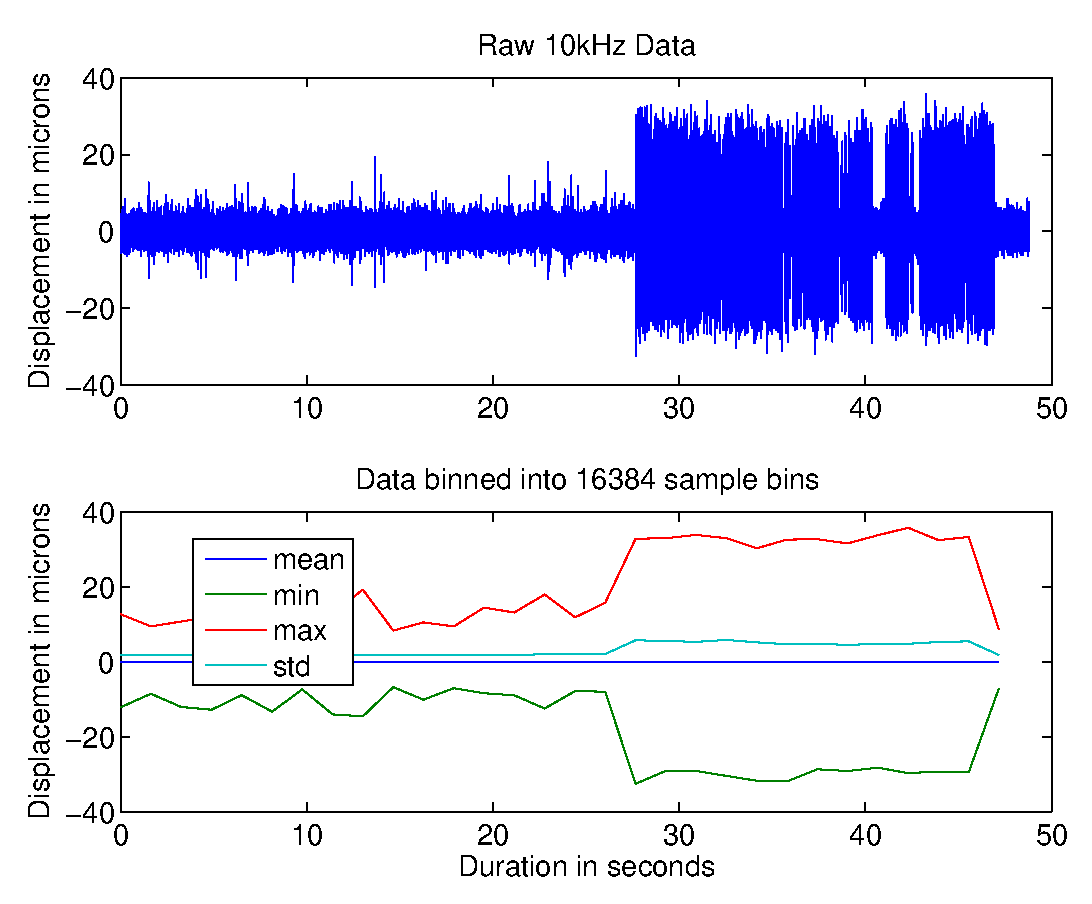
\includegraphics[width=.9\linewidth]{binning}
\end{center}
\end{frame}



\begin{frame}\frametitle{FA Zoomer Matlab Interface}
\includegraphics[width=\linewidth]{fa-zoomer}
\end{frame}



\begin{frame}\frametitle{FA Viewer}
\begin{center}
\includegraphics[width=.85\linewidth]{WEPMN004f6}
\end{center}
\end{frame}



\begin{frame}\frametitle{Spectrum Analysis Tool}
\begin{center}
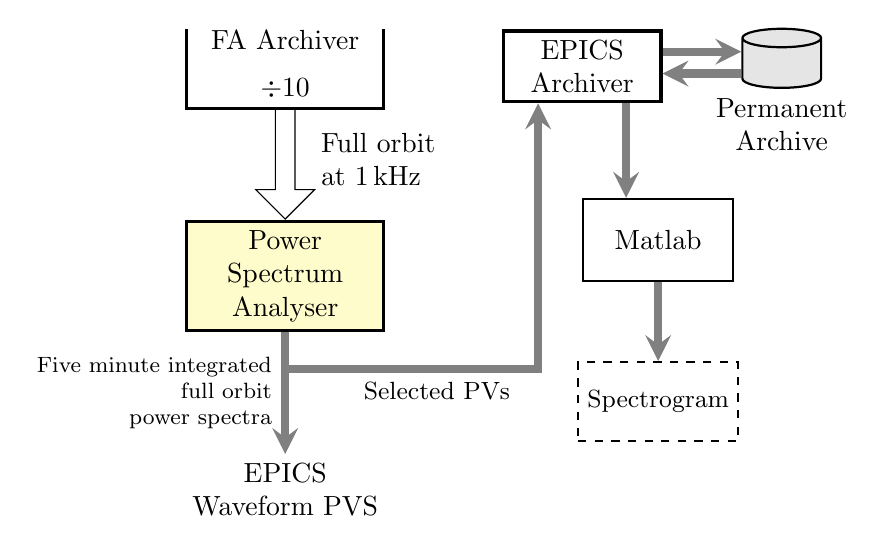
\begin{tikzpicture}

\draw [very thick]
    (0,0) coordinate(ar-nw) -- ++(0,-10mm) --
    ++(25mm,0) coordinate[midway] (ar-s) -- ++(0,10mm) coordinate(ar-ne);
\node [anchor=north, inner sep=0pt] at ($(ar-nw)!.5!(ar-ne)$) {FA Archiver};
\node [anchor=south] at (ar-s) {$\div 10$};

\node [draw, single arrow, rotate=-90, anchor=west, minimum height=14mm,
    label={[align=left, xshift=2mm]above:Full orbit\\at 1\,kHz}]
    (from-archiver) at (ar-s) {};
\node [draw, very thick, anchor=north, align=center, minimum width=25mm,
    fill=yellow!20]
    (analyser) at (from-archiver.east) {Power\\Spectrum\\Analyser};

\node [align=center] (pvs)
    at ($(analyser.south)+(0,-20mm)$) {EPICS\\Waveform PVS};
\draw [gray, line width=3pt, ->] (analyser) -- (pvs)
    coordinate[pos=0.3] (pv nw)
    node [anchor=east, pos=0.5, black, align=right, font=\footnotesize]
    {Five minute integrated\\full orbit\\power spectra};

\node [draw, very thick, align=center, anchor=north west, minimum width=20mm]
    (epics ar) at (40mm,0) {EPICS\\Archiver};
\node [disk icon, anchor=west, xshift=10mm, fill=black!10,
    label={[align=center]below:Permanent\\Archive}]
    (disk) at (epics ar.east) {};
\draw [gray, line width=3pt, ->] (disk.160 -| epics ar.east) -- (disk.160);
\draw [gray, line width=3pt, <-] (disk.190 -| epics ar.east) -- (disk.190);

\draw [gray, line width=3pt, ->] (pv nw) -| (epics ar.-140)
    node [pos=0.3, black, below, font=\small] {Selected PVs};


\node [draw, thick, anchor=north west, inner sep=4mm, yshift=-12mm]
    (matlab) at (epics ar.south) {Matlab};
\draw [gray, line width=3pt, ->]
    (epics ar.-40) -- (epics ar.-40 |- matlab.north);

\node [draw, thick, anchor=north, yshift=-10mm, font=\small, dashed,
    minimum height=10mm]
    (figure) at (matlab.south) {Spectrogram};
\draw [gray, line width=3pt, ->] (matlab) -- (figure);


\end{tikzpicture}

\end{center}
\end{frame}



\begin{frame}\frametitle{Spectrum Analysis Tool: EDM Screen}
\begin{center}
\includegraphics[height=80mm]{spectrum}
\end{center}
\end{frame}



\begin{frame}\frametitle{Spectrogram at one EBPM for a Week}
\includegraphics[width=\linewidth]{spectrogram-3-2}
\end{frame}



% How to skip a block of (valid) code:
\iffalse \fi

\end{document}
